\documentclass{llncs}

\usepackage{amsmath}
\usepackage{amssymb}
\usepackage{amscd}
\usepackage{txfonts}
\usepackage{amsfonts,semantic,colortbl,mathrsfs,stmaryrd}
\usepackage{epsfig,graphicx,subfigure}
\usepackage{enumerate,enumitem}
\usepackage{multirow,multicol}
\usepackage{tabularx}
\usepackage{linearA}
\usepackage{mathabx}
\usepackage{mathrsfs}

\newcommand{\act}[1]{{\xrightarrow{#1}{}}}
\newcommand{\Cao}{\underline{\mbox{\LinearACCCLXXXVI}}}
\newcommand{\Emp}{\underline{[]}}
\newcommand{\Lef}{\underline{[}}
\newcommand{\Rig}{\underline{]}}
\newcommand{\Gc}{{\mathcal{G}^{c}}}
\newcommand{\G}{\mathcal{G}}

\title{Bidirectional Transformation of Querying Ordered Graphs}
\author{Fei Yang}
\institute
{ BASICS\\
  Department of Computer Science and Engineering\\
  Shanghai Jiao Tong University, P.R.China\\
  \email{iamyf@sjtu.edu.cn}
}

\begin{document}
\maketitle

\section{Introduction}\label{sec:intro}

\section{Preliminaries}\label{sec:pre}

Ordered graphs is a graph model in which the branchings are ordered. We start from introducing a formal definition for ordered graphs, and give a bisimilarity equivalence relation on the ordered graphs.

\subsection{Ordered Graphs}\label{subsec:order-graph}

The graphs we treated here are multi-rooted, directed, and edge-labeled graphs with order on outgoing edges. This graph model has three prominent features: \emph{$\epsilon$-edges}, \emph{markers}, and \emph{graph concatenation}. An $\epsilon$-edges represents the a shortcut between two nodes, it is similar with the $\epsilon$-transition in automata. Markers can be treated as interfaces that connect the nodes to other graphs. A node can be marked with \emph{input} and \emph{output markers}. Graph concatenation sequentially aligns two graphs in a given order.

The ordered graph model is formally defined as follows. We write $\mathcal{L}$ for the set of \emph{labels} and $\mathcal{L}_{\epsilon}$ for $\mathcal{L}\cup\{\epsilon\}$. Let $X$ and $Y$ be finite sets of input and output markers; we add the prefix $\&$ for markers like $\& x$.
    An \emph{ordered graph} $G$ is defined by a triple $(V,B,I)$, where
    \begin{itemize}
        \item $V$ is the set of \emph{nodes},
        \item $B:V\rightarrow List(\mathcal{L}_{\epsilon}\times V+Y)$ is a \emph{branch function} mapping a node to a list of \emph{branches}: a branch in $\mathcal{L}_{\epsilon}\times V+Y$ is either a \emph{labeled edge} $\mathbf{Edge}(l,v)$ or an \emph{output marker} $\mathbf{Outm}\&y)$, and
        \item $I:X \rightarrow V$ is a function which determines the \emph{input nodes} (roots) of the graph.
    \end{itemize}

Here, every node in the range of $I$ is called a root. Note that a root node may have incoming edges. However, we can convert it to a equivalent graph having no such incoming edges.

We denote a graph with the input marker set $X$ and the output marker set $Y$ by $G^X_Y$. Moreover, we write $\G^X_Y$ to represent the set of such graphs. Another assumption is that the graphs we are going to talk about are restricted to finite graphs, which means the finiteness on the set of nodes. $\Gc^X_Y$ is used to denote the set of ordered graph with a countble width. It is obvious that the set of finite ordered graphs $\G^X_Y$ is a subset of $\Gc^X_Y$.

For the markers, we allow a graph to have multiple roots. When the graph is single-rooted, we often use $\&$ as the \emph{default marker} to indicate the root and use $\G_Y$ ot denote $G^{\{\&\}}_Y$. 

\subsection{Graph Constructors}\label{subsec:graph-constr}
\begin{figure}[ht]
	\centering
	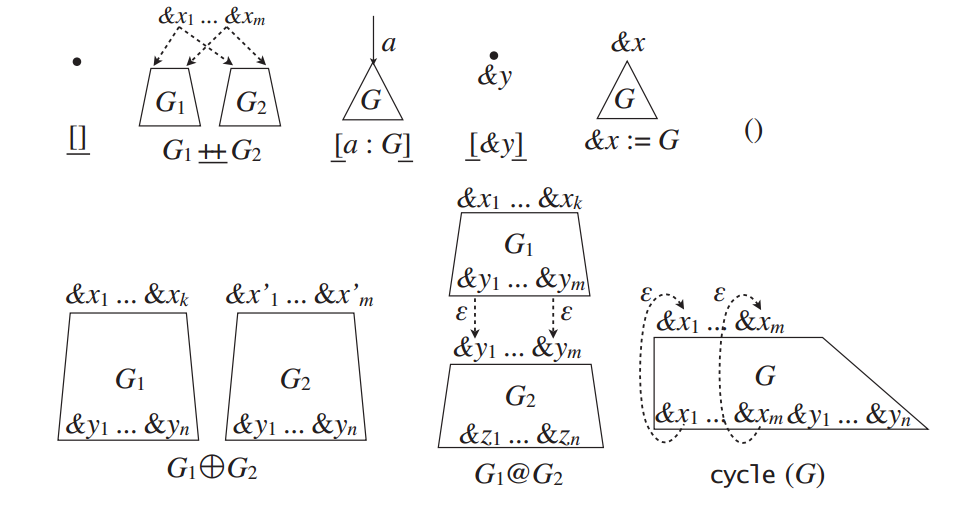
\includegraphics[width=0.8\textwidth]{fig1.png}
	\caption{Graph Constructors}
	\label{fig:graph-constr}
\end{figure}
Figure \ref{fig:graph-constr} sumarizes the nine costructors we used to describe arbitrary graphs.
$$\begin{array}{lcll}
G	&\Coloneqq	&\Emp	&\mbox{\{ single node graph \}}\\
	&\mid	&G_1\Cao G_2	&\mbox{\{ graph concatenation \}}\\
	&\mid	&\Lef a:G\Rig &\mbox{\{ an edge pointing to a graph \}}\\
	&\mid	&\Lef \&y\Rig &\mbox{\{ a node graph with an output marker \}}\\
	&\mid	&\&x\coloneqq G	&\mbox{\{ label he root node eith an input marker \}}\\
	&\mid	&()	&\mbox{\{ empty graph \}}\\
	&\mid	&G_1\oplus G_2	&\mbox{\{ disjoint graph union \}}\\
	&\mid	&G_1 @G_2	&\mbox{\{ append of two graphs \}}\\ 
	&\mid	&\mathbf{cycle}(G)	&\mbox{\{ graph with cycles \}}
\end{array}$$

The single node graph constructor $\Emp$ construct a root-only graph. $G_1\Cao G_2$ adds two $\epsilon$-edges from a new root to the roots of $G_1$ and $G_2$, respectively. $\Lef a:G\Rig$ constructs a graph adding an $a$ labeled edge point to the root of $G$. $\Lef\&y\Rig$ constructs a single node graph with an output marker $\&y$. $\&x\coloneqq G$ associates an input marker $\&x$ to the root node of $G$. $()$ constructs an empty graph with neither a node or an edge. Furthermore, $G_1\oplus G_2$ constructs a graph by using a componentwise $(V,B,I)$ union, $\Cao$ differs from $\oplus$ in that $\Cao$ unifies input nodes while $\oplus$ does not. $\oplus$ requires them to be identical. $G_1 @G_2$ composes two graphs by connecting the output nodes of $G_1$ with the corresponding input nodes of $G_2$ with $\epsilon$ edges. $\mathbf{cycle}(G)$ connects the output nodes of $G$ with the corresponding input nodes with $\epsilon$ edges, that will form cycles. The newly constructed nodes have unique identifiers. The formal definition of the sementics is given in $\lambda_{FG}$. 

\subsection{Proper Branches}\label{subsec:proper-b}

In the definition of ordered graphs, the $\epsilon$-edges are introduced to represent the shortcut between nodes. We need to relate two connected nodes by \emph{proper branch}, where we can ignore the shortcuts. A \emph{proper branch} of a node $v$ is defined as a path from $v$ going through zero or more $\epsilon$-edges until it reaches a non-$\epsilon$-edge or output marker.


Let $G=(V,B,I)\in\Gc^X_Y$ and $v\in V$. The path starting from $v$
$$v(=v_0)\act{\epsilon}_{i_0}v_1\ldots\act{\epsilon}_{i_{n-1}}v_n\act{}_{i_n}$$
is called a \emph{proper branch} of $v$ if the $i_n$-th branch $B(v_n).i_n$ is not an $\epsilon$-edge. (i.e. a non-$\epsilon$-edge or an output marker. The set of all proper branches of $v$ in $G$ is denoted by $Pb(G,v)$. 

Like the order on the branches, a total order is introduced on proper branches. Given two proper branches in an arbitrary graph, $p=(v\act{\epsilon}_{i_0}v_1\ldots\act{\epsilon}_{i_{n-1}}v_n\act{}_{i_n})$, and $p'=(v\act{\epsilon}_{i_0'}v_1'\ldots\act{\epsilon}_{i_{n'-1}'}v_{n'}'\act{}_{i_{n¡¯}'})$. Let their branch index sequences be $\tilde{p}\stackrel{def}{=}(i_0,\ldots,i_{n-1},i_n)$ and $\tilde{p'}\stackrel{def}{=}(i_0',\ldots,i_{n'-1}',i_{n'}')$. We define $p\leq_{Pb}p' \stackrel{def}{\Longleftrightarrow}\tilde{p}\leq_l\tilde{p'}$ where $\leq_l$ is the lexicographical order between branch index sequences. This order plays an important roll in the definition of bisimilarity and the procedure of bidirectionalizing elimination of $\epsilon$-edges.

For a given proper branch $p$, we use $p.last$ to denote the last step of the branch sequence, which is either a non-$\epsilon$ edge or a output marker.

\subsection{Bisimilarity for Ordered Graphs}\label{subsec:bis}

For the soundness of the graph model, we need an equivalence relation that can judge whether two arbitrary graphs are the same. At first glimpse, graph isomophism is the most straight forward approach. However, it is not necessarily that two graphs are isomophic when they behaves the same. Another option is language equivalence, which is focused on the language produced by the graphs, But unfortunately, it is proved to be undecidable in automata theory. Semantic equivalence is widely used in program verification to overcome the above difficulties. Bisimilarity is a kind of semantic equivalence, which is focused on the observable behavior of the graphs. 

On unordered graphs, we use the notion of value equivalence (Bisimilarity) as the equivalence relation used in verfication. A similar bisimilarity on ordered graphs is given.

For two graphs $G=(V,B,I)$and $G'=(V',B',I')$ in $\Gc^X_Y$, a relation $R$ between $V$ and $V'$ is called a \emph{bisimulation relation}, if for any $vRv'$, there is an order isomorphism $f:(Pb(G,v),\leq_{Pb})\rightarrow(Pb(G',v'),\leq_{Pb})$ satisfying he following order-preserving property: For any proper branch $p=(v\act{\epsilon}_{i_0}v_1\ldots\act{\epsilon}_{i_{n-1}}v_n\act{}_{i_n})\in Pb(G,v)$ with $f(p)=(v\act{\epsilon}_{i_0'}v_1'\ldots\act{\epsilon}_{i_{n'-1}'}v_{n'}'\act{}_{i_{n'}'})\in Pb(G',v')$, we have
\begin{itemize}
    \item Edge Correspondence: if $B(v_n).i_n=\mathbf{Edge}(l,u)$ for some $l\in\mathcal{L}, u\in V$, then  $\exists u'\in V'$ s.t. $B'(v_{n'}').i_{n'}'=\mathbf{Edge}(l,u')$ and $uRu'$,
    \item Marker Correspondence: if $B(v_n).i_n=\mathbf{Outm}(\&y)$ for some $\&y\in Y$, then $B'(v_{n'}').i_{n'}'=\mathbf{Outm}(\&y)$.
\end{itemize}
Two graphs $G$ and $G'$ are \emph{bisimilar} (denoted by $G\sim G'$) if there is a bisimulation relation $R$ s.t. for every input marker $\&x\in X$, $I(\&x)RI'(\&x)$.

The notion of bisimilarity only consider the reachable part of a given graph. This means the unreachable parts are disregarded, i.e. two bisimilar garphs are still bisimilar if one adds subgraphs unreachable frome input nodes.

\section{$\lambda_{FG}$: A Transformation Language for Ordered Graphs}\label{sec-lambda}

\subsection{The Core $\lambda_{FG}$}\label{subsec:core}

$\lambda_{FG}$ is a transformation language for transforming (querying) ordered graphs. There is a formal semantics for constructing and querying an ordered graph in $\lambda_{FG}$. It is an extenstion of typed $\lambda$-calculus with graph constructors and list functions. It has a powerful feature of structural recursion. It is capable of querying with manipulating the sibling of nodes, which gives a great expresiveness power to the language. The syntex of $\lambda_{FG}$ is given as below. It also has a system of strictly defined type inference rules.
$$\begin{array}{lclr}
\sigma	&\Coloneqq	&\sigma\rightarrow\sigma\mid\sigma+\sigma\mid\sigma\times\sigma	& \mbox{\{ function, coproduct, product types \}}\\
	&\mid	&\mathbf{List}(\sigma)\mid\mathbf{Bool} &\mbox{\{ list and boolean types \}}\\
	&\mid	&\mathbf{Label}\mid\mathbf{G}^X_Y	&\mbox{\{ label and graph types \}}\\
\\
e	&\Coloneqq	&x\mid\lambda x.e\mid e\,e\mid\mathbf{case}\,e\,\mathbf{of}\,\mathbf{in_l}(x)\rightarrow e\,\mathbf{or}\,\mathbf{in_r}(y)\rightarrow e	&\\
	&\mid	&\mathbf{in_l}e\mid\mathbf{in_r}e\mid(e,e)\mid\mathbf{pr_l}e\mid\mathbf{pr_r}e	&\mbox{\{ terms of lambda calculus \}}\\
	&\mid	&\mathbf{nil}\mid\mathbf{cons}(e,e)\mid\mathbf{foldr}(e,e)\mid\ldots &\mbox{\{ functions for lists \}}\\
	&\mid	&\mathbf{if}\,e\,\mathbf{then}\,e\,\mathbf{else}\,e	&\mbox{\{ conditional \}}\\
	&\mid	&a|e=e	& \mbox{\{ labels $(a\in\mathcal{L})$ and label equality \}}\\
	&\mid	&\Emp\mid e\Cao e\mid \Lef e:e\Rig\mid\Lef\&y\Rig\mid\&x\coloneqq e\mid()\mid e\oplus e	&\\
	&\mid 	&e @ e\mid \mathbf{cycle}(e)	&\mbox{\{ graph constructors \}}\\
	&\mid	&\mathbf{isEmpty}(e)	&\mbox{\{ graph emptiness checking \}}\\
	&\mid	&\mathbf{srec}(e,e)	&\mbox{\{ structural recursion functions \}}
\end{array}$$

Here we focus on the explaination of \emph{structural recursion}, which is a powerful graph transformation mechanism. It provides the capability to descirbe the queries and transformations that garantees the termination of the computation and preserves the finiteness.

In general the structure recursion is written of the form $\mathbf{srec}(e,d)$, wherer $e$ can be considered as the body function applied on the labeled edges and $d$ is a map computation on nodes. For a simple case, we can consider $d=\mathbf{foldr}(\odot,\iota_{\odot})$ for some monoid $(\odot,\iota_{\odot})$ on $\mathbf{G}^Z_{Z\times\alpha}$. The structural recursion function $f\stackrel{def}{=}\mathbf{srec}(e,d)$ satisfies the following equations (herer, equality means bisimilarity):
$$\begin{array}{lcl}
f(\Emp)	&=&	\iota_{\odot}\\
f(g_1\Cao g_2)	&=&	f(g_1)\iota f(g_2)\\
f(\Lef l:g\Rig)	&=&	e(l,g) @ f(g)\\
f(\&x\coloneqq g)	&=&	(\oplus_{\&z\in Z}(\&z,\&x)\coloneqq\Lef(\&z,\&\Rig)@f(g)\\
f(())	&=&	()\\
f(g_1\oplus g_2)	&=&	f(g_1)\oplus f(g_2)
\end{array}$$

\begin{example}\label{ex:a2dxc}
This example shows how to manipulate edges of the graph and change its shape by structural recursion, The following function $a2d\_xc$ replaces all labels $a$ with $d$ and contracts $c$-labeled edges. 
$$\begin{array}{lll}
a2d\_xc	&=\mathbf{srec}(rc,\mathbf{foldr}(\Cao,\Emp))&	\\
	&\mathbf{where}\,rc(l,g)=	&\mathbf{if}\,l=a\,\mathbf{then}\,\Lef d:\Lef\&\Rig\\
	&	&\mathbf{else}\,\mathbf{if}\,l=c\,\mathbf{then}\,\Lef\&\Rig\,\mathbf{else}\,\Lef l:\Lef\&\Rig\Rig
\end{array}$$
\end{example}

Compared with the structural recurcion in UnCAL, structural recurtion in $\lambda_{FG}$ can deal with orered graphs and computations on the sibling dimension of graphs. This ability is given by the function of $d$. 

\subsection{Bulk Semantics of Structural Recursion}\label{subsec:bulk}

The structural recursion of $\lambda_{FG}$ has two equivalent semantics. One is \emph{recursive semantics}. It defines the function behavior and the program transformation/optimization recursively. It appears to be more concise and is useful for reasoning. Another one is \emph{bulk semantics}. By allowing $\epsilon$-edges, we can evaluate a structural recursion in a \emph{bulk} manner. The bulk semantics consider the transformation on a whole. It is useful in parallel computation and the proof of termination and finiteness-preserving property. In the construction of bidirectional semantics, we will also apply the bidirectionlization on bulk semantics.

Before the introduction of bulk semantics, let us consider the type of the structural recursion function $\mathbf{srec}(e,d)$ in advance. A type inference rule is given below.

$$\inference{\vdash e:\mathbf{Label}\times\mathbf{G}_Y\rightarrow\mathbf{G}^Z_Z \vdash d:\mathbf{List}(\mathbf{G}^Z_{Z\times\alpha}+\mathbf{G}^Z_{Z\times Y})\rightarrow\mathbf{G}^Z_{Z\times\alpha+Z\times Y}}{\vdash\mathbf{srec}(e,d):\mathbf{G}^X_Y\rightarrow\mathbf{G}^{Z\times X}_{Z\times Y}}$$

Here, $e$ is the body function of the transformation on edges. it performs a similar role as the body function in the unordered version. It maps the a subgraph of a labeled edge into the result graph. For the $d$ function, it works as a rearrangement function over the lists. It maps the each lists by manipulate the order of the branches. In the bulk semantics, the evaluation can be applied in parallel. It mainly involves three steps.
\begin{enumerate}
	\item Map computation on edges with $e$: the function $e$ is applied on each labeled edge, yield a set of intermediate result graphs for $e$. The set graphs will be rearranged in the next step.
	\item Map computation on nodes with $d$: the function $d$ is applied on each nodes. The previous set of graphs are merged by the rearrangement measure defined in $d$, leads to a set of merged graphs for each node.
	\item Groups new graphs with $\epsilon$-edges: to get the final result, the graphs for each node need to be grouped by $\epsilon$-edges. The $\epsilon$-edges are added according to the input and output markers of the previous result. 
\end{enumerate}

\section{An Overview of Bidirectional Transformation}\label{sec:overview}

In UnCAL, there is a framework that could bidirectionalize unordered graph transformation. It consists of a two stage bidirectionalizing strategy and it could solve the problem that the graphs may contain shared nodes or cycles. This framework provides us a some heuristic idea to do the bidirectionalizing on $\lambda_{FG}$. 

The challenging parts of bidirectionalizing on $\lambda_{FG}$ comes from the $d$ function in the structural recursion. It leads to a three step bulk semantics, which would make it hard to trace back from the view. Further, the $d$ function only accepts graphs without $\epsilon$-edges. Thus, an $\epsilon$-elimination procedure has to be applied before the structural recursion for an arbitrary graph. Also, the $\epsilon$-edge should be eliminated before it is presented to the customer. Moreover, the order of the branchings must be treated carefully in our bidirectionalization. 

\subsection{Bidirectional Properties}\label{subsec:b-prop}

The goal in bidirectionalizing $\lambda_{FG}$ is to approach the bidirectionalization in ordered graphs by providing a bidirectional semantics in $\lambda_{FG}$. The semantics should have bidirectional properties defined in the previous work in UnCAL. Let $\mathscr{F}\ldbrack e\rdbrack\rho$ denote a forward evaluation (get) of expression $e$ under environment $\rho$ to produce a view, and $\mathscr{B}\ldbrack e\rdbrack(\rho,G')$ denote a backward evaluation (put) of expression $e$ under environment $\rho$ to reflect a possibly modified view $G'$ to the source by computing an updated environment. An \emph{environment} $\rho$ is a mapping with a form $\{\$x\mapsto X,\ldots\}$ where $X$ is a graph $G$ or a label $l$, and $\$x$ is a variable. The transformation need to satisfy the following two important properties:

$$\inference{\mathscr{F}\ldbrack e\rdbrack\rho=G}{\mathscr{B}\ldbrack e\rdbrack(\rho,G)=\rho}(GETPUT)\quad
\inference{\mathscr{B}\ldbrack e\rdbrack(\rho,G')=\rho' \mathscr{F}\ldbrack e\rdbrack\rho'=G''}{\mathscr{B}\ldbrack e\rdbrack(\rho,G'')=\rho'}(WPUTGET)$$

The (GETPUT) property states that unchanged view $G$ should give no change on the environment $\rho$ in the backward evaluation, while the (WPUTGET) property states that the modified view $G'$ and the view obtained by backward evaluation followed by forward evaluation may differ, but both view have the same effect on the original source if backward evaluation is applied. A pare of forward and backward evaluation is \emph{well-behaved} if it satisfies (GETPUT) and (WPUTGET) proties. In the rest of the paper, the forward and backward evaluations will be presented for $\lambda_{FG}$, and the following theorem holds.

\begin{theorem}[Well-behavedness]\label{th:wellb}
The proposed forward and backward evaluations are well-behaved, provided their evaluations succeed.
\end{theorem}

According to the (WPUTGET) property, given a certain forward evaluation function, there could be more than one backward evaluation that would satisfy the well-behavedness property. When we perform the modification on the view, the most reasonable choice is to reflet it on the corresponding part on the source. This is the \emph{location correspondence} property. Moreover, the modification on the view graph could be categorised into three types: in place updates, edge deletion and edge insertion. In order to maintain the well-behavedness between the updated source and the modified view, we also need to apply some operation on the source. A reasonable assumption is that a certain type of modification on the view yields the same type of operation on the source, which could be called the \emph{operation correspondence} property.

\begin{theorem}[Rationality]\label{th:rat}
The proposed bidirectional transformation on $\lambda_{FG}$, satisfies both location and operation correspondence property. We call it a rational transformation.
\end{theorem}

The rationality property is also important as it gives us a discriptive goal in designing the bidirectionalizing the transformation. The goal is to let the updates on the source to meet the intention of the changing on the view.

\subsection{Three-Stage Bidirectionalization}\label{subsec:3-sta}

In an arbitrary transformation, there could be a big gap between the source and view graoh. It makes it hard to reflect changes on the view to the source. The basic idea to divide the forward evaluation into three stages, each one could be bidirectionalized.
\begin{itemize}
	\item Stage 1: Elimination of $\epsilon$-edges on the source, to produce a simple source that we can apply bulk semantics on it.
	\item Stage 2: Forward evaluation using bulk semantics. This stage may create some new $\epsilon$-edges, so that the output graph will have a similar shape to the input graph. Appropriate trace information might be appended locally on the nodes in the result graph.
	\item Stage 3: Elimination of $\epsilon$-edges to produce a usual view.
\end{itemize}

In our bidirectional transformation framework, we will propose a general bidirectionalized $\epsilon$-edge elimination procedure for both Stage 1 and Stage 3. For Stage 2, a bidirectionalized semantics for $\lambda_{FG}$ is provided in this paper. Thus, the whole transformation is bidirectionlized by a inductively defined procedure.

\section{Bidirectionalizing $\epsilon$-elimination procedure}\label{sec:eps}

In the previous work of $\lambda_{FG}$, the input graph of the $d$ function in structural recursion does not accept any $\epsilon$-edges. However, we can not safely assume that an arbitrary input graph does not contain any $\epsilon$-edges. Further, after applying the transformation via bulk semantics, some $\epsilon$-edges might be introduced to maintain the structure of the result graph. In most applications, $\epsilon$-edges are assumed to be unobservable. Thus, we wish to produce a view without any $\epsilon$ to the users. In this seciton, a bidirectionalized $\epsilon$-elimination procedure is proposed. 

First, there is an effective procedure that whether the $\epsilon$-elimination could be applied successfully on a finte ordered graph $G$. The details could be found in the paper of $\lambda_{FG}$.

\begin{lemma}\label{lamma:eps-exists}
Given an finite ordered graph $G$ possibly with $\epsilon$-edges, there is an effective procedure to decide whether there exists an ordered graph $G'$, s.t. $G\sim G'$ and has neither $\epsilon$-edges nor infinite width. If yes, produce such $G'$.
\end{lemma}

The idea of the $\epsilon$-elimination procedure is to use labeled edges to connect the shortcut between proper branches, the procedure is defined as below. Note that we use a list of integers to represent the total orders over the branches and proper branches on a node.

\begin{definition}\label{def:epsilon}
For a graph $G=(V,B,I)\in\Gc^X_Y$, the $\epsilon$-elimination $\epsilon\mbox{-elim}(G)$ of $G$ is a graph $(V,B'I)\in\Gc^X_Y$ where $|B'(v)|\stackrel{def}{=}Pb(G,v)$, and $B'(v).\tilde{p}\stackrel{def}{=}Pb(G,v).\tilde{p}.last$ for $p=(v\act{\epsilon}_{i_0}\ldots v_n\act{}_{i_n})$ in $B'(v)$.
\end{definition}

Next we will introduce how to reflect view updates within $\epsilon\mbox{-elim}(G)$ to the source graph $G$. We will use the correspondence between the proper branches in the source graph and the branches in the view graph.

\begin{enumerate}
	\item For the inplace-updates on an arbitrary edge $B'(v).\tilde{p}\in\epsilon\mbox{-elim}(G)$, the corresponding labeled edge on the view is $Pb(G,v).\tilde{p}.last$. We could apply the same update operation on this edge. 
	\item For the edge deletion on an arbitrary edge $B'(v).\tilde{p}\in\epsilon\mbox{-elim}(G)$, we update the source graph by delete the correcponding edge $Pb(G,v).\tilde{p}.last$.
	\item For the edge insertion, since the set of nodes $V$ is the same on the view and the source. Thus, we just need to insert the edge to the same place on the source.
\end{enumerate}

After we have done the update operation on the source, an $\epsilon$-elimination procedure need to be applied again on the updated source. The reason is that, the updated labeled edge may be duplicated in different proper branches. Thus, the corresponding edge of these proper branches on the view graph also need to be updated to mainain the consistency between the source and the view. For inplace updates and edge deletion, the corresponding edge is deleted on the view, and for edge insertion, the edge is added according to the newly added proper branches. Therefore, the whole procedure would satisfy the well-behavedness. Moreover, the rationality is also infered from this constructive bidirectionalizing procedure.

\begin{lemma}\label{lemma:well-epsilon}
The proposed bidirectionalized $\epsilon$-elimination procedure satisfy the well-behavedness and the rationality property.
\end{lemma}

\section{Traceble Forward Evaluation}\label{sec:fwd}

Practically, a $\lambda_{FG}$ expression usually specifies a forward transformation that maps a source ordered graph (possibly a database or an XML file) to a view graph. A backward transformation for this procedure specifies how to reflect view updates to the source graph. However, the structural information kept by $\epsilon$-edges will not appear explicitely in the view graph. Moreover, the newly created parts within the transformation procedure also make it hard to detect the generated source for everything in the view graph. In this sence, some appropriate trace information should be added to the view, to make the view more informative, in other words, \emph{traceable}. In this section, we will enrich the original semantics of $\lambda_{FG}$ to make it produces traceable view after forward transformation.

\subsection{Local Trace Information}\label{subsec:local}

Recall the semantics in $\lambda_{FG}$, a view is obtained by evaluating a $\lambda_{FG}$ expression with an ordered graph. Every node in the view graph is either a graph obtained from the source graph, or a node constructed by te $\lambda_{FG}$ expression, except the node generated through a structural recursion(in bulk semantics). For an arbitrary structural recursion function $\mathbf{srec}(e_1,d)(e_2)$, the input of the body function $e_1$ is evaluated binding variables from a part of evaluated result in $e_2$; and the input of the rearrangement $d$ function is evaluated by binding variables from the result in $e_1$. So the node in the result graph may originate from not only the whole $srec$ expression but also a sub-expression in $e_2$. Thus, a more complicated inductively defined trace information should be added on the nodes on the result graph.

Here, we use the a \emph{traceable view} in which each node has information for tracing its origin. This locally added information, called $TraceID$, is defined by

$$\begin{array}{lll}
TraceID &\coloneqq	&SrcID\\
	&\mid		&Code\,Pos\,Marker\\
	&\mid		&RecN\,Pos\,TraceID\,Marker\\
	&\mid		&RecE\,Pos\,TraceID\,TraceID\,Num\\
	&\mid		&RecM\,Pos\,Marker\,TraceID\,Num\\
	&\mid		&RecD\,Pos\,TraceID\,TraceID
\end{array}$$

\subsection{Enriched Forward Semantics}\label{subsec:fwd-sem}


\section{Backward Evaluation}\label{sec:bak}

\subsection{Reflection of Inplace Updates}\label{subsec:bak-inp}

\subsection{Reflection of Edge Deletion}\label{subsec:bak-del}

\subsection{Reflection of Edge Insertion}\label{subsec:bak-ins}
\section{Conclusion}\label{sec:con}

\end{document}
